\chapter{Results}


Describe the initial conditions, table, cool


\section{BEM alligned rotor \textcolor{red}{BERNAT}}


\subsection{Main outputs \textcolor{red}{BERNAT}}


\subsubsection{Angle of attack and inflow angle \textcolor{red}{BERNAT}}

\subsubsection{Axial and azimuthal inductions \textcolor{red}{BERNAT}}

\subsubsection{Thrust and azimuthal loading \textcolor{red}{BERNAT}}

\subsubsection{Total thrust and torque \textcolor{red}{BERNAT}}


\section{BEM yawed rotor \textcolor{blue}{NIKLAS}}


\subsection{Main outputs \textcolor{blue}{NIKLAS}}


\subsubsection{Angle of attack and inflow angle \textcolor{blue}{NIKLAS}}

\subsubsection{Axial and azimuthal inductions \textcolor{blue}{NIKLAS}}

\subsubsection{Thrust and azimuthal loading \textcolor{blue}{NIKLAS}}

\subsubsection{Total thrust and torque \textcolor{blue}{NIKLAS}}

\section{Influence of the tip correction \textcolor{green}{CARLOS}}

The results shown in this section were obtained for the rotor described in the assignment instructions, operating with a tip speed ratio $ \lambda = 8 $ and no yaw. It can be seen that the tip correction reduces the power and thrust, resulting in a worse performance. Indeed, the rotor without the tip correction has a higher $ C_P/C_T $ ratio.

Near the blade tip, the flow angle $ \phi $ is reduced due to the tip vortex (Figure \ref{img:tc-phi}), because it induces a larger axial velocity (Figure \ref{img:tc-a}). Having a lower flow angle $ \phi $ results in a reduced power extraction, which is proportional to $ c_l \sin \phi - c_d \cos \phi $ (Figure \ref{img:tc-dcp-dmu}) \cite{weh-ch3}. However, reducing the flow angle $ \phi $ contributes to an increase of the thrust, since it is proportional to $ c_l \cos \phi + c_d \sin \phi $.

Note that $ c_l $ also decreases due to the reduction of $ \phi $, because it implies a decrease of the angle of attack $ \alpha $ (Figure \ref{img:tc-alpha}). Moreover, the relative velocity, which also affects the loads, will also be larger for the case without tip correction.

The tip correction tries to account for this effect. The expression Prandtl derived for that factor is shown in equation \ref{eq:f-prandtl}. Its value over the blade is plotted in Figure \ref{img:tc-f}.

\begin{equation}
f(\mu) = \frac{2}{\pi} \arccos \left[ \exp \left( - \frac{B}{2} \left( \frac{1-\mu}{\mu} \right) \sqrt{1+\frac{\lambda^2\mu^2}{(1-a)^2}} \right) \right]
\label{eq:f-prandtl}
\end{equation}

\begin{itemize}
	
	\item Power coefficient $ C_P $
	\begin{itemize}
		\item Tip correction: 0.4528
		\item No tip correction: 0.4757
		\item Increase: 5.05 \%
	\end{itemize}
	
	\item Thrust coefficient $ C_T $
	\begin{itemize}
		\item Tip correction: 0.6581
		\item No tip correction: 0.6691
		\item Increase: 1.67 \%
	\end{itemize}
	
	\item Power to thrust ratio $ C_P/C_T $
	\begin{itemize}
		\item Tip correction: 0.6880
		\item No tip correction: 0.7109
		\item Increase: 3.32 \%
	\end{itemize}
	
\end{itemize}

\begin{figure}[htbp]
	\centering
	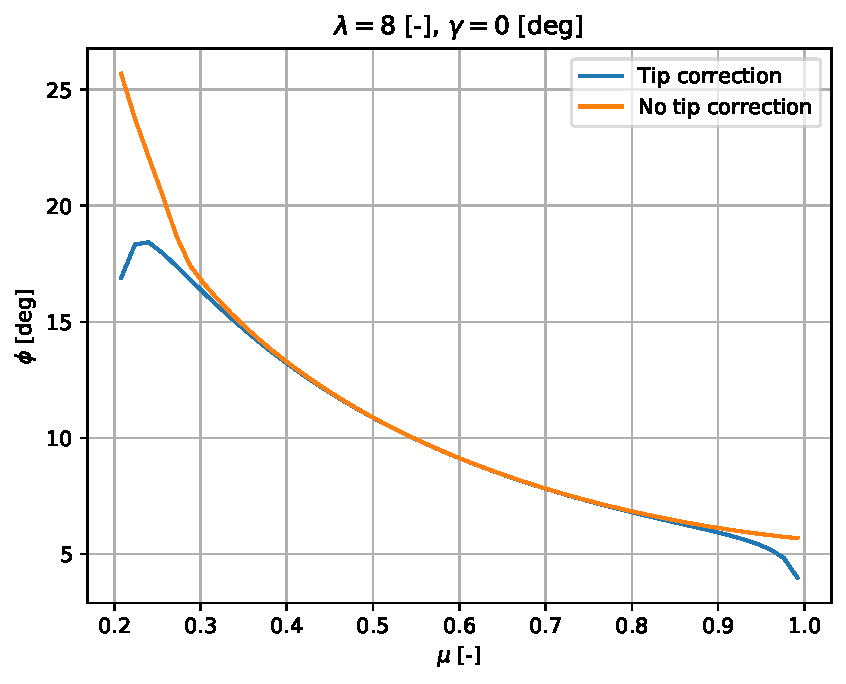
\includegraphics[height=0.45\textheight]{./img/tip-correction/phi.pdf}
	\caption{Flow angle distribution with and without tip correction.}
	\label{img:tc-phi}
\end{figure}

\begin{figure}[htbp]
	\centering
	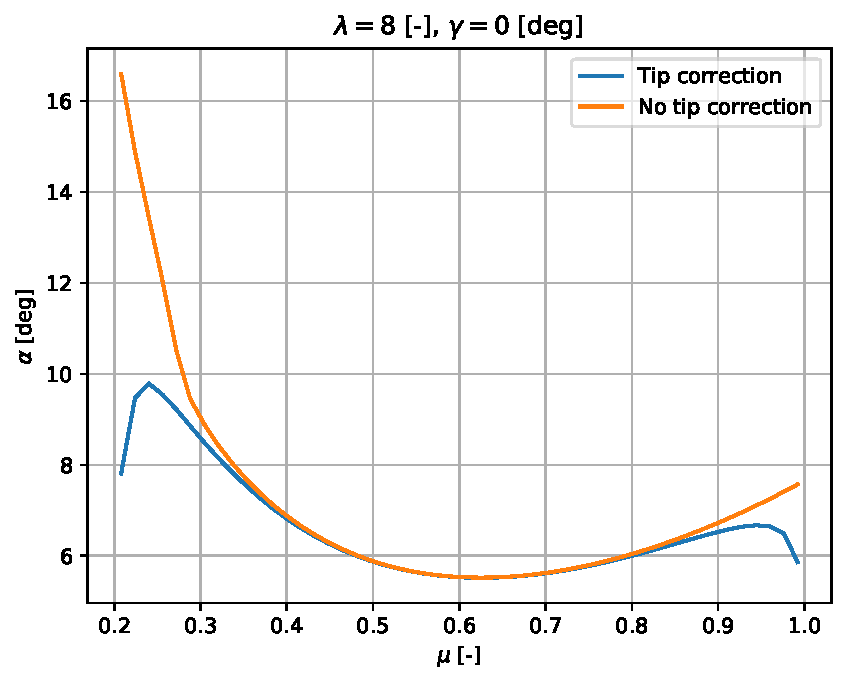
\includegraphics[height=0.45\textheight]{./img/tip-correction/alpha.pdf}
	\caption{Angle of attack distribution with and without tip correction.}
	\label{img:tc-alpha}
\end{figure}

\begin{figure}[htbp]
	\centering
	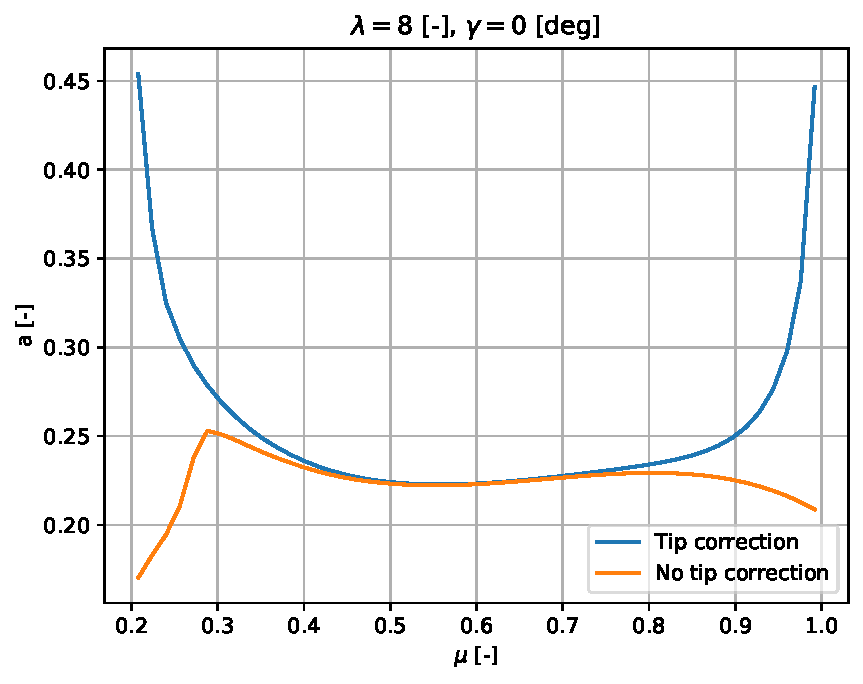
\includegraphics[height=0.45\textheight]{./img/tip-correction/a.pdf}
	\caption{Axial induction distribution with and without tip correction.}
	\label{img:tc-a}
\end{figure}

\begin{figure}[htbp]
	\centering
	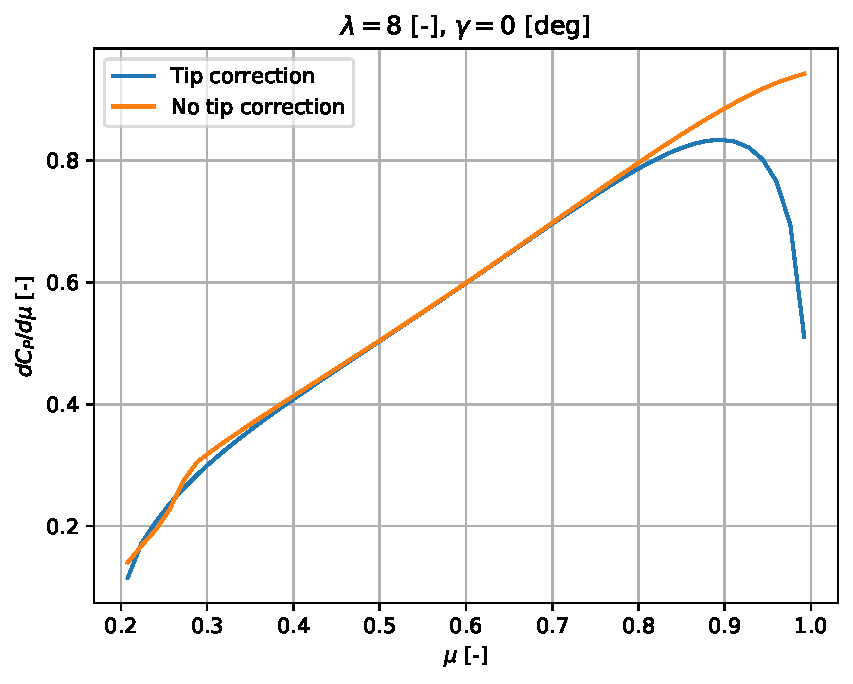
\includegraphics[height=0.45\textheight]{./img/tip-correction/dcp_dmu.pdf}
	\caption{Power coefficient distribution with and without tip correction.}
	\label{img:tc-dcp-dmu}
\end{figure}

\begin{figure}[htbp]
	\centering
	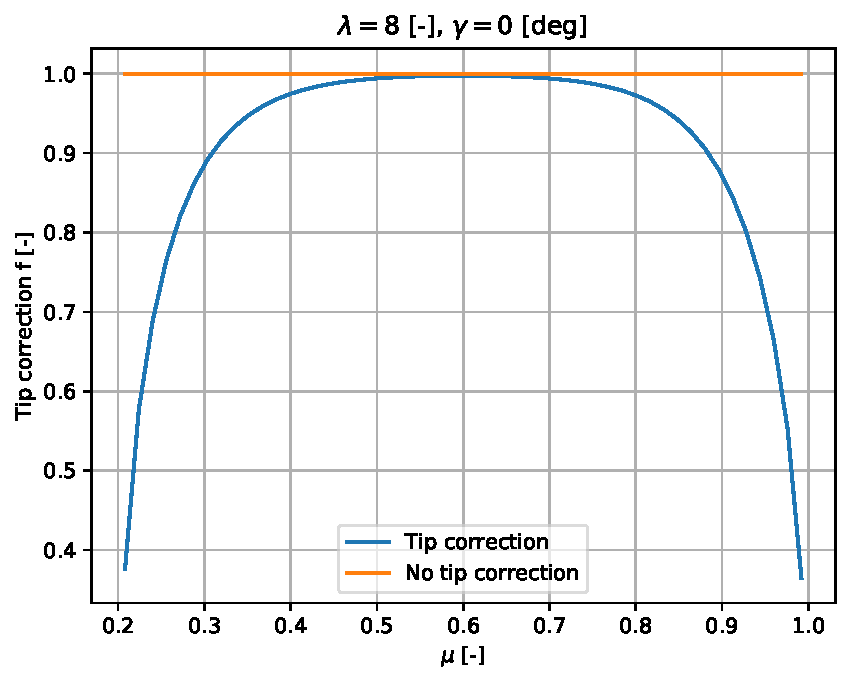
\includegraphics[height=0.45\textheight]{./img/tip-correction/f.pdf}
	\caption{Prandtl's tip loss factor distribution with and without tip correction.}
	\label{img:tc-f}
\end{figure}

\section{Influence of numerical discretization \textcolor{red}{BERNAT}}

\section{Evaluation of stagnation enthalpy \textcolor{green}{CARLOS}}

Plot the distribution of stagnation enthalpy as a function of radius at four locations: infinity upwind, at the rotor (upwind side), at the rotor (downwind side), infinity downwind.

\section{System of circulation and vorticity \textcolor{green}{CARLOS}}

Plot a representation of the system of circulation. Discuss the generation and release of vorticity in relation to the loading and circulation over the blade.

\section{Operational point \textcolor{blue}{NIKLAS}}
